\section{Arquitectura de la Solución}

\subsection{Visión General de la Arquitectura}

La arquitectura propuesta para el sistema KUYA-UNICEF se basa en un enfoque modular y escalable que garantiza la flexibilidad, mantenibilidad y rendimiento del sistema. La solución adopta una arquitectura de microservicios con patrones modernos de desarrollo.

\begin{figure}[h]
\centering
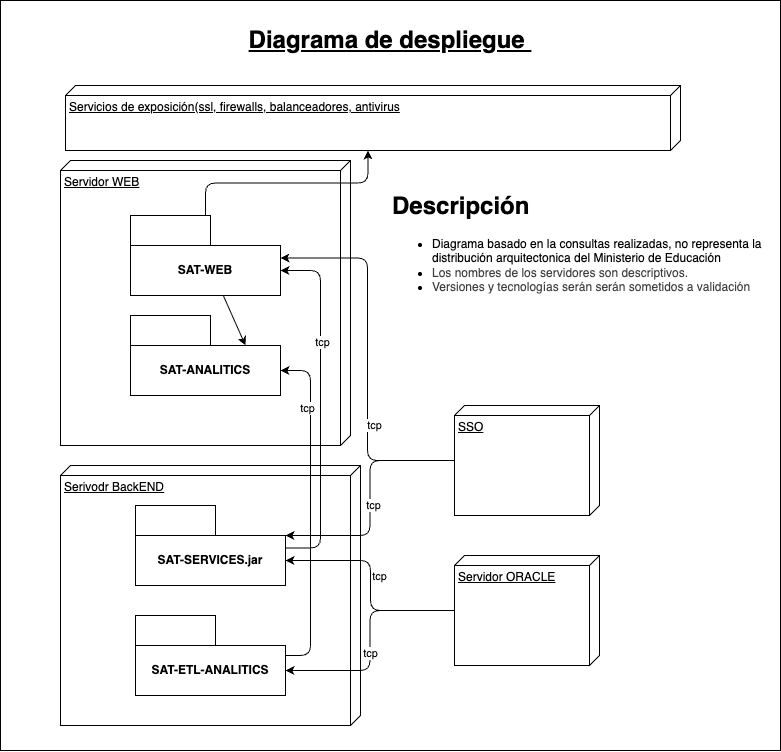
\includegraphics[width=0.8\textwidth]{graficos/arquitectura.png}
\caption{Propuesta de Diagrama de Arquitectura de la Solución SAT}
\label{fig:arquitectura}
\end{figure}

\subsection{Componentes Principales}
En continuidad con los productos existentes expuestos en los terminos de referencia, la arquitectura se compone de los siguientes módulos principales:

\subsubsection{Capa de Presentación}
En continuidad con las tecnologias indicadas en los terminos de referencia, las implmementaciones propuestas incluyen:
\begin{itemize}
    \item \textbf{Integracion SSO}: Implementar la autenticación única (SSO) utilizando el sistema existente en el Ministerio de Educación, cultura y deporte.
    \item \textbf{Frontend Web}: Aplicación Angular con manejo de autenticación y autorización basado en roles RBAC, con diseño adaptable para tablets y dispositivos móviles.
    \item \textbf{Dashboard de Monitoreo}: Visualización interactiva de datos y alertas en tiempo real, utilizando bibliotecas como D3.js o Chart.js.
    Implmetación de Dashboard interactivo avanzado desarrollado con streamlit de python.
\end{itemize}

\subsubsection{Capa de Servicios}
\begin{itemize}
    \item \textbf{API Gateway}: Punto de entrada único para todas las solicitudes basadas en servicios RESTful, gestionando la seguridad y el enrutamiento, documentación con Swagger.
    \item \textbf{Balanceador de Carga}: Distribución eficiente del tráfico, mediante el uso de NGINX
    \item \textbf{Servicio de Autenticación}: Gestión de usuarios y permisos, basado en OAuth2 y JWT, integrándose con el SSO existente.
    \item \textbf{Servicio de Datos}: Procesamiento de los datos para la generación de analisis y reportes, generando una base de datos de analisis intermedia.
    \item \textbf{Servicio de Notificaciones}: Alertas y comunicaciones
\end{itemize}

\subsubsection{Capa de Datos}
\begin{itemize}
    \item \textbf{Base de Datos Principal}: PostgreSQL para datos transaccionales
    \item \textbf{Data Warehouse}: Para análisis y reportes históricos
    \item \textbf{Cache}: Redis para optimización de rendimiento
\end{itemize}

\subsection{Tecnologías Propuestas}
En continuidad de las tecnologias indicadas en los terminos de referencia, se propone el siguiente stack tecnológico:

\begin{table}[h]
\centering
\begin{tabular}{|l|l|}
\hline
\textbf{Componente} & \textbf{Tecnología} \\
\hline
Backend & Java Spring \\
Frontend & Angular \\
Base de Datos & ORACLE \\
MenCache & Redis \\
CI/CD & GitLab CI \\
\hline
\end{tabular}
\caption{Stack Tecnológico Propuesto}
\label{tab:stack_tecnologico}
\end{table}

\subsection{Versionamiento y Despliegue}

Para el desarrollo de la solución se utilizará git como herramienta de versionamiento, teniendo ramas de desarrollo, pruebas, piloto y producción.

El método de despliegue será ajustado a los métodos actuales del Ministerio de Educación, cultura y deporte, asegurando una integración fluida con los sistemas existentes, de no existir una método establecido, se propone la implementación de pipelines de CI/CD utilizando GitLab CI para automatizar pruebas y despliegues.